\subsection{Prima riunione}
\label{sec:prima-riunione}
Lo scopo della prima riunione è stato quello di discutere la proposta del committente e permettere al core team del progetto di conoscere il dominio del caseificio. Il committente ha messo a disposizione la propria sala riunioni per tre ore per svolgere il primo incontro.
Su suggerimento di Linda, si è deciso di adottare la tecnica dell'\emph{Event Storming}~\cite{cit:event-storming} per condurre la riunione.

\subsubsection{Partecipanti}
\label{sec:prima-riunione-partecipanti}
\begin{itemize}
  \item Linda (facilitatore)
  \item Giacomo, Nicolò e Nicolas (membri del core team)
  \item Raffaella (proprietaria del caseificio e responsabile pianificazione)
  \item Gianluca (responsabile ordini e addetto vendite)
  \item Simone (casaro e responsabile produzione)
  \item Luisa (responsabile magazzino)
\end{itemize}

\subsubsection{Setup}
\label{sec:prima-riunione-setup}
Sebbene il committente abbia fornito la sala riunioni per tutta la mattinata (dalle 9:00 alle 12:00) il team ha segnato le 9:30 come orario di inizio effettivo per avere il tempo di preparare in maniera opportuna la sala.
Infatti, questa presenta la classica disposizione con un grande tavolo al centro circondato da sedie. Secondo Brandolini, padre dell'Event Storming, questo è un ``anti pattern'': infatti, porta i partecipanti a pensare che il meeting si svolgerà come tutte le altre (noiose) riunioni aziendali dove una persona parla e gli altri stanno seduti ad ascoltare~\cite[pp.~116-118]{cit:event-storming-book}.

L'approccio dell'Event Storming vuole puntare su una forte interazione fra i diversi esperti dei settori aziendali per approfondire la conoscenza del dominio e allo stesso tempo far emergere i veri bisogni del cliente. Per ottenere questo risultato si organizza la riunione in modo da sorprendere i partecipanti incentivandoli a una partecipazione attiva.

Quindi è stato appeso un grande rotolo di carta lungo tutta una parete della sala e sono stati messi a disposizione numerosi blocchetti di post-it colorati e pennarelli come mostrato in \Cref{fig:event-storming-setup}. Inoltre, il grande tavolo è stato spostato dal centro della stanza e le sedie sono state impilate per scoraggiare che i partecipanti si siedano durante la riunione diventando degli osservatori passivi.

\begin{figure}[!ht]
  \centering
  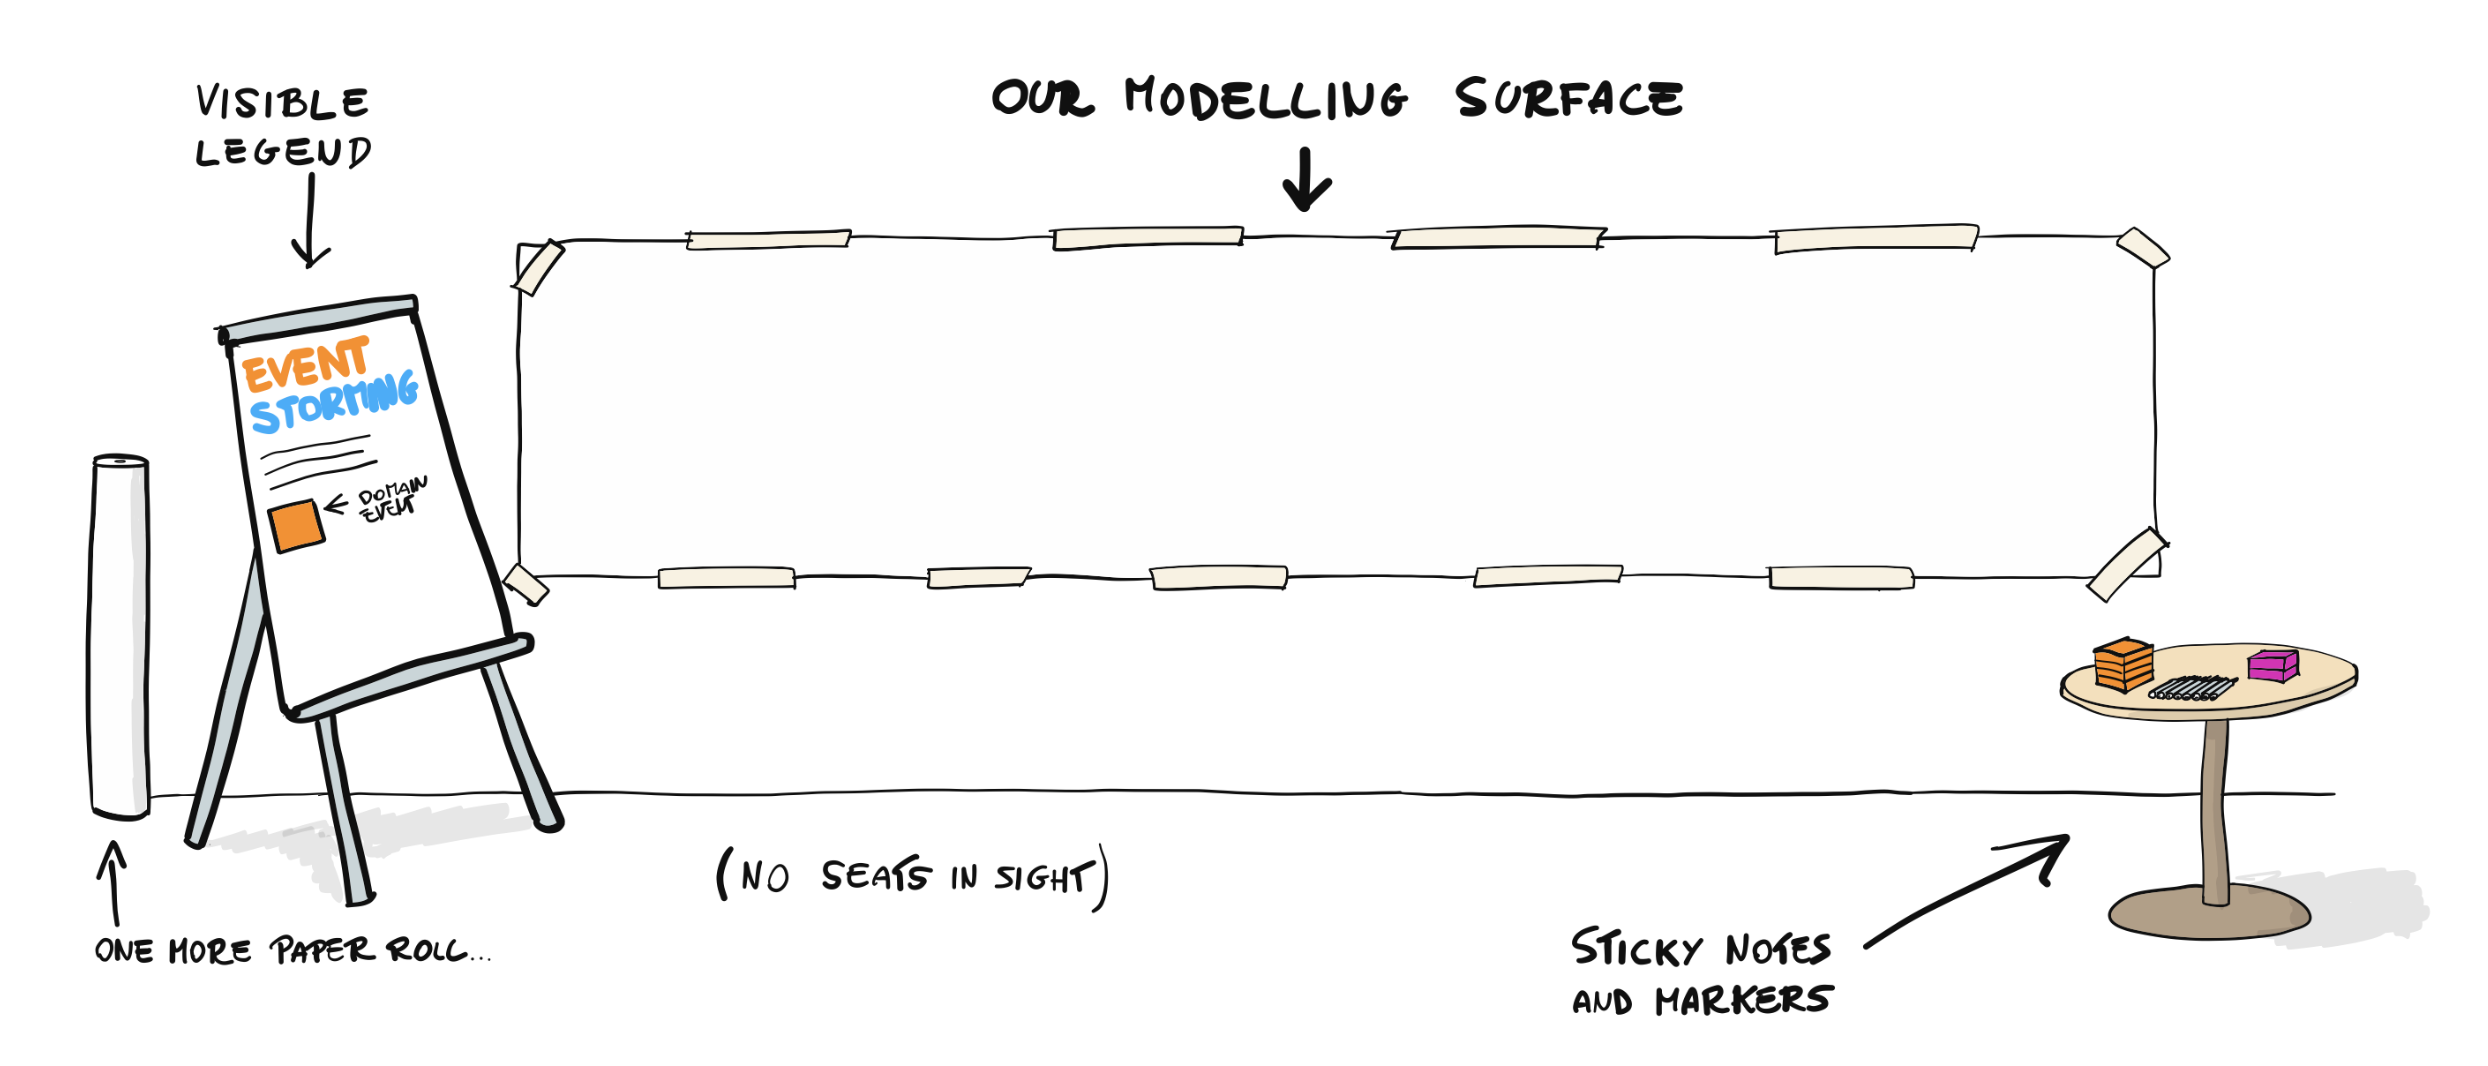
\includegraphics[width=0.8\textwidth]{images/event-storming-setup.png}
  \caption{Preparazione per una sessione di Event Storming}
  \label{fig:event-storming-setup}
\end{figure}

\subsubsection{Kick off}
\label{sec:prima-riunione-kick-off}
Intorno alle 9:30 è iniziata la riunione; si poteva notare che i partecipanti erano spaesati ma allo stesso tempo incuriositi dal grande rotolo di carta.
Linda, nel ruolo di facilitatore, ha lanciato il meeting con un breve giro di presentazioni.
Successivamente, ha spiegato in maniera esplicita l'obiettivo della riunione in modo che fosse chiaro a tutti i partecipanti.

\begin{tabularx}{.9\textwidth}{rX}
  \speak{Linda} & L'obiettivo di questo incontro è analizzare gli attuali processi aziendali del caseificio per cercare di capire come possano essere migliorati e automatizzati interagendo armonicamente fra loro e con sistemi preesistenti. All'inizio il processo potrebbe sembrarvi difficile ma vi invito a intervenire senza paura, qualunque cosa facciate sarà utile. \\
\end{tabularx}

La spiegazione del facilitatore è volutamente molto breve: non si vuole annoiare con una lunga descrizione ma lasciare che gli esperti di dominio inizino subito a descrivere il loro lavoro. L'importante è che il facilitatore trasmetta una sensazione di sicurezza e disponibilità ad aiutare i partecipanti.

\begin{tabularx}{.9\textwidth}{rX}
  \speak{Linda}     & Vorrei che descriveste degli eventi rilevanti al vostro ambito aziendale su questi post-it arancioni e che li attacchiate in ordine cronologico sul rotolo di carta. \\
  \speak{Raffaella} & Potresti spiegare meglio cosa intendete con ``eventi''?                                                                                                              \\
  \speak{Linda}     & Certamente! Ti faccio un esempio concreto: lavoro nel settore degli ordini, un evento che mi interessa è quando ricevo via email un nuovo ordine.                    \\
                    & \emph{Mentre parla, Linda scrive la frase ``Nuovo ordine ricevuto per email'' su un post-it arancione}                                                               \\
  \speak{Raffaella} & Ah, adesso mi è chiaro... quindi un evento che mi interessa potrebbe essere ``Fatto nuovo piano di produzione''?                                                     \\
  \speak{Linda}     & Esatto! L'importante è che nel descrivere l'evento usiate sempre un verbo al passato come ha fatto adesso Raffaella.                                                 \\
\end{tabularx}

\subsubsection{Esplorazione caotica}
\label{sec:prima-riunione-esplorazione-caotica}

I primi minuti di una riunione di Event Storming sono sempre i più difficili: i partecipanti potrebbero essere spiazzati dalla nuova modalità di interazione e fare fatica a individuare degli eventi da scrivere sui post-it.
È fondamentale in momenti come questo il facilitatore dia loro supporto ma non li guidi attivamente; nel caso in cui non sia presente una persona coraggiosa in grado di rompere il ghiaccio attaccando il primo post-it, potrebbe farlo il facilitatore con un esempio.
Fortunatamente, in questo caso Raffaella ha già chiaro cosa scrivere e attacca per prima un post-it alla parete.

\begin{tabularx}{.9\textwidth}{rX}
  \speak{Linda} & Ottimo, grazie Raffaella! Come vedete basta che scriviate eventi rilevanti per il settore aziendale dove lavorate. Non ci sono risposte sbagliate, scrivete tutto quello che vi viene in mente. \\
\end{tabularx}

Spesso potrebbero formarsi dei piccoli gruppetti di persone che si confrontano per scegliere il termine più adatto da scrivere sui post-it. È compito del facilitatore cercare di ``spezzare'' questi gruppetti per evitare che continue discussioni riducano il flusso di post-it e che non emergano elementi contraddittori fondamentali all'analisi del dominio.

Il modello inizia a prendere forma, il numero di post-it attaccati cresce rapidamente e i partecipanti si sentono sempre più a proprio agio. Potrebbero esserci diversi post-it duplicati o incongruenze, ciò è perfettamente normale, anzi non bisogna cercare la perfezione in questa fase.

\subsubsection{Controllo della coerenza del risultato}
\label{sec:prima-riunione-controllo-della-coerenza-del-risultato}

Quando il flusso di post-it inizia a diminuire ed emerge una timeline approssimata è il momento adatto per passare alla seconda fase. Il risultato ottenuto dalla prima fase, come mostrato in \Cref{fig:event-storming-exploration}, può presentare post-it duplicati e cluster all'interno di un flusso disorganizzato. Questo punto di partenza verrà rifinito in modo da far sì che venga rispettata correttamente la timeline del dominio e che possa emergere un modello coerente.

\begin{figure}[!ht]
  \centering
  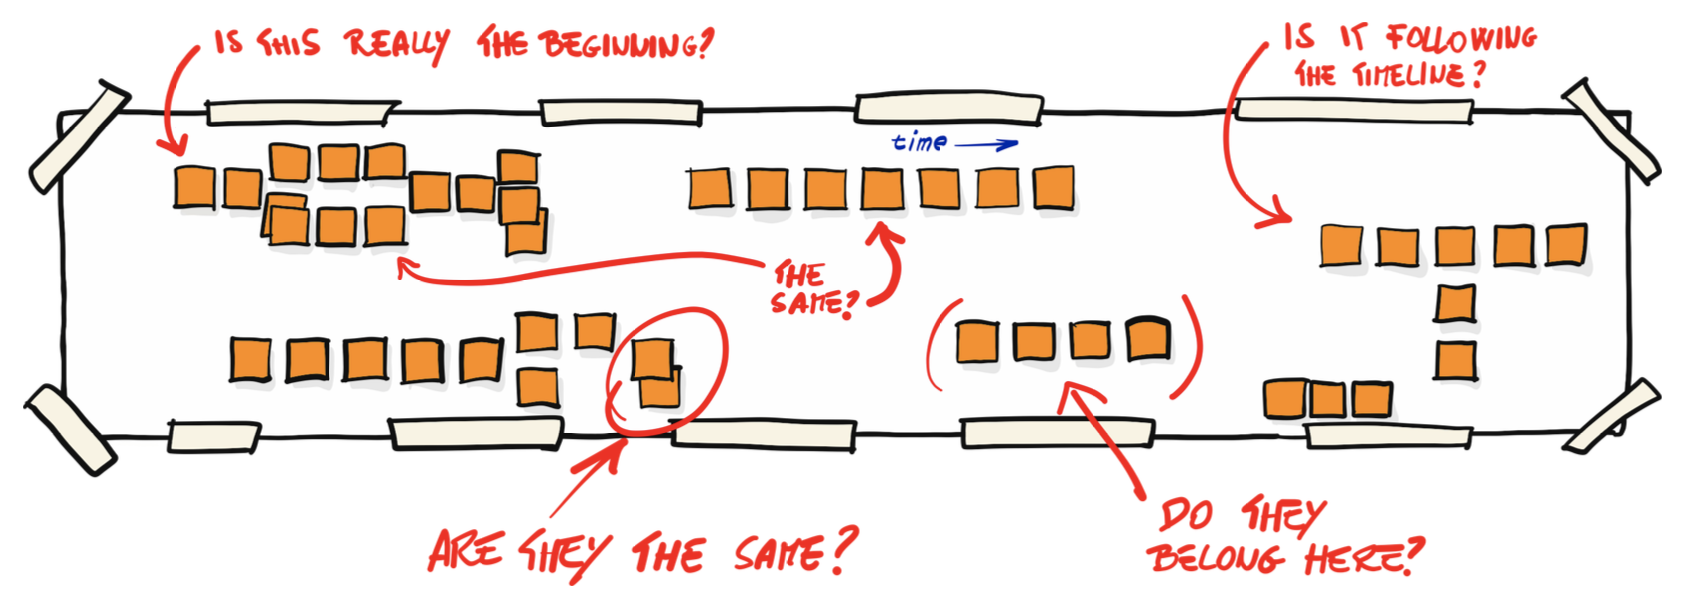
\includegraphics[width=0.8\textwidth]{images/event-storming-exploration.png}
  \caption{Esempio di come può apparire il modello ottenuto dalla prima fase di esplorazione caotica}
  \label{fig:event-storming-exploration}
\end{figure}

Per riordinare i vari cluster di eventi è utile individuare le cosiddette \emph{swimlanes}: suddivisioni logiche dei vari eventi raggruppandoli in base a omogeneità per attori o dipartimenti aziendali interessati. \Cref{fig:event-storming-swimlanes}

\begin{figure}[!ht]
  \centering
  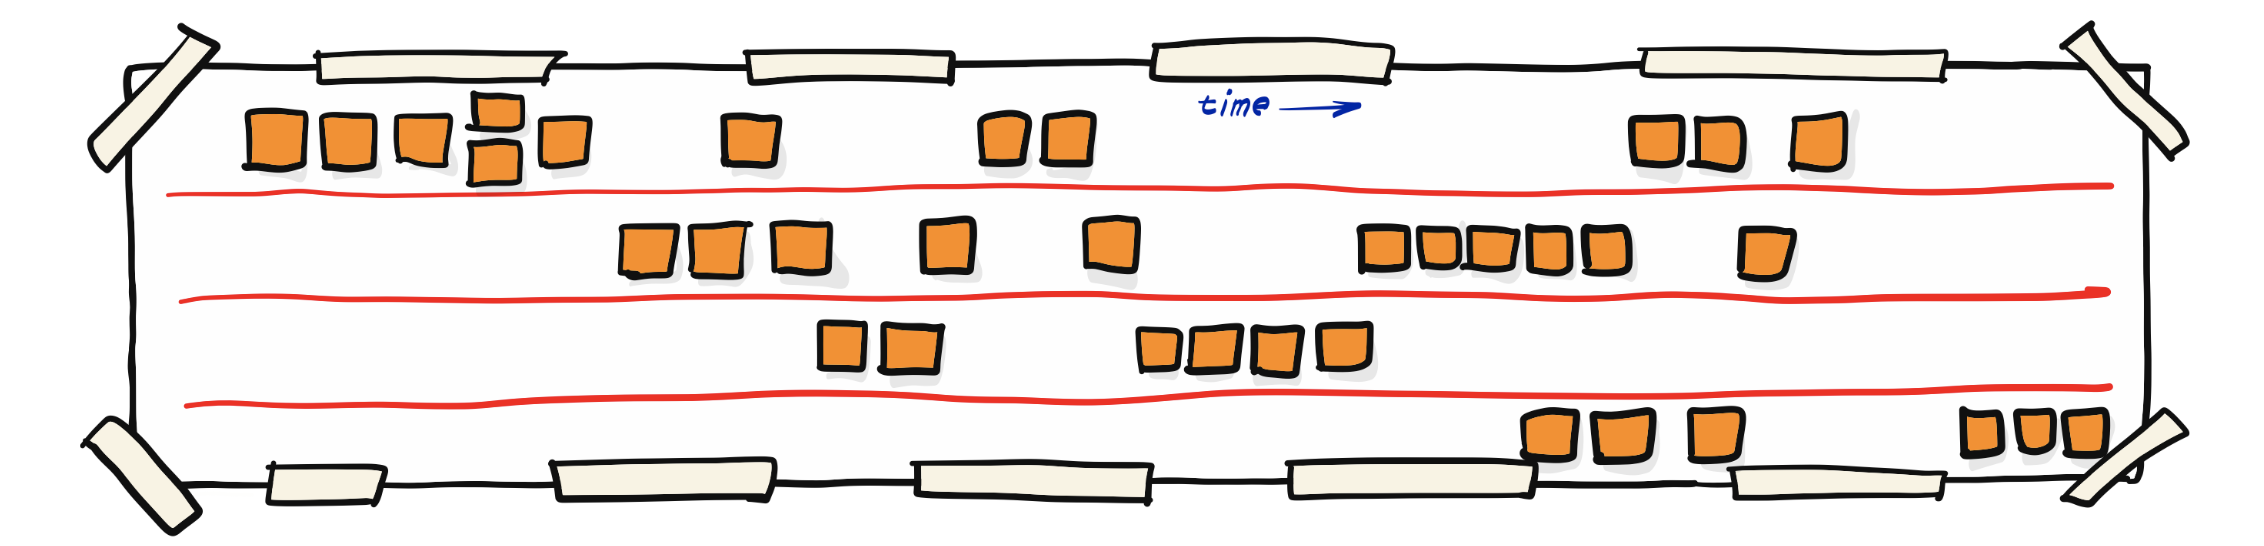
\includegraphics[width=0.8\textwidth]{images/event-storming-swimlanes.png}
  \caption{Esempio di individuazione di swimlanes}
  \label{fig:event-storming-swimlanes}
\end{figure}

Riordinare gli eventi in maniera coerente comporterà il confronto fra esperti di diversi settori aziendali; spesso potrebbero emergere delle incongruenze nel modo in cui i vari silos interpretano gli eventi. Queste discussioni sono fondamentali per individuare i punti dove sono presenti delle criticità nell'interazione fra i dipartimenti; il facilitatore non deve farsi sfuggire tali discussioni e marcare con appositi post-it viola i punti dove è necessario un ulteriore approfondimento.

\subsubsection{Persone e sistemi esterni}
\label{sec:prima-riunione-persone-e-sistemi-esterni}

Una volta che il modello è stato riordinato si possono inserire per ogni flusso di eventi le persone (o attori, per utilizzare la terminologia UML) che vi interagiscono.

\begin{tabularx}{.9\textwidth}{rX}
  \speak{Linda}    & Ora vi chiedo di indicare, per i flussi di eventi di vostra competenza quali sono le persone che avviano tale flusso e che vi interagiscono.                                                  \\
                   & \emph{Nel mentre Linda disegna su un post-it giallo una versione stilizzata di Raffaella con sotto scritto il suo nome e lo attacca all'inizio del flusso di pianificazione della produzione} \\
  \speak{Gianluca} & Quindi visto che io gestisco gli ordini dovrei mettermi all'inizio di quel flusso?                                                                                                            \\
  \speak{Linda}    & Esatto, potremmo metterci anche un generico ``cliente'' visto che è lui che fa partire effettivamente l'ordine e tutto il flusso che lo gestisce.                                             \\
\end{tabularx}

Una volta inserite le persone si può fare lo stesso in maniera analoga con i sistemi esterni con cui un flusso deve interagire.
Nel nostro caso, il sistema della tracciabilità è un sistema esterno:

\begin{tabularx}{.9\textwidth}{rX}
  \speak{Linda}    & mi sembrava di avervi sentito discutere di un sistema della tracciabilità che usate per i vostri prodotti.                                                                                                        \\
  \speak{Gianluca} & Sì, è un sistema esterno che dobbiamo utilizzare per garantire la tracciabilità in caso ci siano problemi con dei lotti.                                                                                          \\
  \speak{Linda}    & Bene, allora potremmo aggiungere anche questo sistema al nostro schema.                                                                                                                                           \\
                   & \emph{Mentre parla linda scrive ``Sistema tracciabilità'' su un post-it rosa e lo attacca vicino agli eventi che vi devono interagire}                                                                            \\
  \speak{Gianluca} & Purtroppo questo sistema è molto scomodo da usare, ogni volta che devo inserire un nuovo lotto perdo tantissimo tempo; purtroppo il sistema dev'essere usato da tutti e non possiamo modificarlo o metterci mano. \\
                   & \emph{Linda non si lascia sfuggire questa osservazione fondamentale e annota subito il problema con un post-it viola}                                                                                             \\
  \speak{Linda}    & Grazie Gianluca per l'osservazione, è un problema su cui potremo tornare a discutere, per il momento lo annoto così.                                                                                              \\
                   & \emph{Linda attacca sotto al post-it del sistema tracciabilità un altro post-it viola con scritto ``Scomodo da usare, fa perdere troppo tempo!''}                                                                 \\
\end{tabularx}

\subsubsection{Walkthrough esplicito}
\label{sec:prima-riunione-walkthrough-esplicito}
Terminati i passaggi precedenti si svolge un \emph{walkthrough} esplicito dove si scorrono evento per evento tutti i post-it per verificare un'ultima volta che non ci siano incongruenze o problemi. Anche in questo caso il facilitatore deve guidare i partecipanti e lasciare che siano loro a fare il racconto evento per evento; infatti, sono loro gli esperti che possono individuare eventuali incongruenze. Se fosse il facilitatore a rileggere gli eventi potrebbe trascurare elementi importanti che invece non sfuggirebbero a un esperto di dominio.

\subsubsection{Problemi e opportunità}
\label{sec:prima-riunione-problemi-e-opportunità}
Avendo a disposizione un modello completo e coerente dei processi aziendali è ora possibile individuare ulteriori \emph{pain point} che non siano già emersi in precedenza e eventuali idee di miglioramento dei processi.

\begin{tabularx}{.9\textwidth}{rX}
  \speak{Linda}     & Molto bene, adesso vi darò questi post-it viola e vi chiederei di annotare tutti i problemi che vi vengono in mente con l'attuale schema dei vostri processi aziendali. \\
  \speak{Raffaella} & Per me sarebbe utilissimo un sistema per fare la pianificazione della produzione in maniera automatica!                                                                 \\
                    & \emph{Raffaella attacca un post-it con scritto a grandi lettere ``Automatizzare'' vicino al flusso di pianificazione della produzione}.                                 \\
\end{tabularx}

Questi punti sono essenziali per poter comprendere ciò di cui ha veramente bisogno il committente e poterlo aiutare a migliorare i processi aziendali.

\subsubsection{Conclusione}
\label{sec:prima-riunione-conclusione}
La riunione è terminata dopo un paio d'ore di lavoro e il \emph{deliverable} prodotto è il grande cartellone con tutti i post-it che descrive accuratamente i processi aziendali, le loro interazioni, gli attori che vi partecipano e i punti critici che necessitano migliorie.
Questo artefatto sarà fondamentale come punto di partenza per le riunioni successive.

Questa prima riunione ha avuto anche il grande beneficio di permettere ai membri del core team che vi hanno preso parte di comprendere meglio i processi aziendali che dovranno andare a modellare. Tale conoscenza è fondamentale per permettere un rapido sviluppo del software e per evitare di andare a creare un sistema che non risponda alle esigenze del cliente.

Il documento prodotto -- il cartellone con i post-it -- è riportato in \Cref{app:cartellone-event-storming} e tutto il processo che ha portato alla sua realizzazione può essere visto al \href{https://youtu.be/BvkPYtI8MF8}{seguente video}.
